\chapter{教小孩统计分析} % Introduction chapter suppressed from the table of contents

``过去半年，我们几个团队在每次迭代回顾时都统计了一些数据，总共有70多条，后面有什么数据分析？''\\
``你们的目的是什么？''我问。\\
``希望预测下一轮迭代的工作量。''\\
``确实可以利用项目历史数据做预测，但请问你记得以前高中学过的统计吗？''\\
``统计学很高深啊！我都还给数学老师了。''\\
``若要深入了解和研究统计分析，确实要具备很好的根底，但如果只是应用------利用统计分析解决日常的问题，便简单多了。统计里有很多可用的工具，虽然不用深究背后的原理，但还是要知道怎样应用。以下是我如何教小孩统计分析的故事。''\\

\hypertarget{ux4eceux8003ux8bd5ux6210ux7ee9ux5f00ux59cb}{%
\subsection{从考试成绩开始}\label{ux4eceux8003ux8bd5ux6210ux7ee9ux5f00ux59cb}}

孩子：爸爸，你是做什么工作的？我明天要在班上介绍自己父母的工作。\\
我：帮客户做统计分析。\\
孩子：统计分析？\\
我心里想你这初中孩子，要如何给你解释统计分析呢？\\
我尝试用一个他可以想象的场景来介绍------假如下面是你班里同学的数学成绩，你会用什么方式把这些成绩表达出来？\\
孩子有点迷茫。\\
=== 20名学生在数学考试中的分数(满分为100分，按大小排序) ===

30, 35, 37, 40, 40, 49, 51, 54, 54, 55\\
57, 58, 60, 60, 62, 62, 65, 67, 74, 89

我：任何样本数据，都可以用图加平均值、范围等来表达。\\
举例：我们可以画茎叶图(Stem and Leaf Plot)(详见附件)表达这些学生成绩：\\
\href{文件:MA_FA2_1.0.1.jpg}{文件:MA FA2 1.0.1.jpg}\\
把20组数从最低排到最高。排在第十的学生和第十一的学生的平均数56，叫中位数(Median)。排第五和第六成绩的平均值44.5，就是Q1（1/4）。排第十五名和第十六名的平均值62，就是Q3（3/4）。\\
这个例子中茎叶图再加上Q1、Q2(中位数)、Q3，{[}44.5、56、62{]}便可以总括表达这20名学生的成绩分布。也可以用下面的柱状图/直方图表达：\\
\href{文件:MA_FA1_1-1.jpg}{500px}

也可以利用 Q1、Q2、Q3(四分位数)画箱线图来表达(详见附件)。\\
除了中位数，也常用平均值(Mean)来表示数据的中间趋势，平均值就是把所有数据加起来，然后把总数除以数量，比如上面20名学生数学成绩的平均值是......\\
孩子充满自信，打断我说：这个平均值简单，我懂。\\
我说：好啊，你这么懂平均值，我问你一个小问题？\\
\{\textbar{} class="wikitable" \textbar{} 问题：5、10、350、355
的平均数是多少？

\textbar{}\}

孩子拿了计算器算出：180。\\
我：你知道那些数是代表什么吗？\\
孩子：不知道。\\
如果这些数是代表角的度数，它的平均值应该是零，而不是180。这是统计分析很重要的概念------你必须知道那些数的背景，否则你的分析没意义。如果你把那4个数字当成是距离来算均值是180，与4个角度数求均值的结果就完全不一样了。\\
从以上例子，你就知道了解问题背景(Context)很重要。\\
孩子：这些统计分析有什么用？\\
我：例如有了这成绩的分析，你就可以知道自己的成绩在整个班是处于什么位置？也可以帮你比较不同科目的成绩。

\hypertarget{ux6bd4ux8f833ux79cdux6559ux5b66ux65b9ux6cd5}{%
\subsubsection{比较3种教学方法}\label{ux6bd4ux8f833ux79cdux6559ux5b66ux65b9ux6cd5}}

45名学生被随机分成5个大小相同的组。两组(A、B)采用目前使用的方法(控制组)，另外3组(C、D、E)采用3种新方法。实验结束时，所有学生参加了一次标准测试，结果(满分30分)见表1。关于教学方法的差异，可以得出什么结论?\\
表1

\resizebox{\linewidth}{!}{

\renewcommand{\arraystretch}{1.5}

\begin{tabular}{|c|c|c|c|c|c|c|c|c|c|}
\hline
\multicolumn{10}{|c|}{45名学生的测试结果 }\\
\hline
A组(控制组)&17&14&24&20&24&23&16&15&24\\
\hline
B组(控制组)&21&23&13&19&13&19&20&21&16 \\
\hline
C组(赞赏组)&28&30&29&24&27&30&28&28&23\\
\hline
D组(责骂惩罚组)&19&28&26&26&19&24&24&23&22\\
\hline
E组(不理睬组)&21&14&13&19&15&15&10&18&20\\
\hline
\end{tabular}

}

我：你可以用刚学过的四分位数(Q1、Q2、Q3)配合箱线图表示每一组数据分布，然后看看有没有差异。这样你便可以比较5个班的成绩。\\
他过了15分钟就画了5个组的箱线图：\\
\href{文件:箱线图1.jpg}{500px}

我：能看到显著区分吗？\\
孩子：看得出是C组最好，D组也比较好，E组就比较差。\\
我：是的，但如果我们只是比较5个组成绩的平均值，没有考虑每一班成绩范围，便不能全面比较。例如：上面数学考试成绩的Q1、Q2、Q3是（44.5、56、62），如果C组的数学成绩是（32、57.5、63），你会认为C组比你们好吗？虽然中位数比你们班高，但Q1比你们低很多，所以不能单看中位数（或平均值）比较。

看到他对这些挺有兴趣，我便问他如何表达以下数据。\\

\hypertarget{ux4ebaux4e00ux5e74ux5185ux9605ux8bfbux6708ux520aux7684ux6570ux91cf}{%
\subsubsection{20人一年内阅读月刊的数量}\label{ux4ebaux4e00ux5e74ux5185ux9605ux8bfbux6708ux520aux7684ux6570ux91cf}}

0, 1, 11, 0, 0, 0, 2, 12, 0, 0\\
12, 1, 0, 0, 0, 0, 12, 0, 11, 0

我看他开始使用同样方法，
我便说这些统计数据跟前面学生成绩的分布不一样，它一头一尾最高，这表示大部分人要么就是不看杂志，要么就是每个月都看，这种分布就不合适用刚才那些方法去表达，只能说它有两个高峰，或者叫众数(Mode)，再配上一个柱状图。如果我们用中位数或者这些数的平均值，或三分位数来表达的话，反而是误导读者，不能正确的表达那些数据的分布。\\
%\href{文件:MA_FA4_1.0.png}{文件:MA FA4 1.0.png}\\

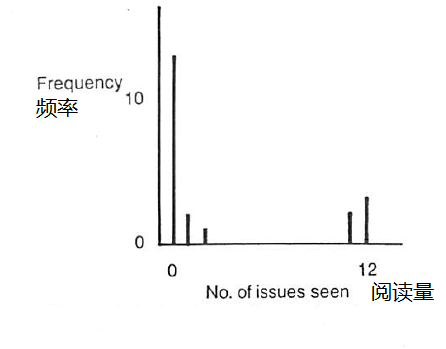
\includegraphics[width=10cm]{MA_FA4_10.png}
当总体(Population)包含非常多数据时，就只能抽样，用抽样来估计Population分布。但是要注意，如果样本不是随机抽样(Random
Sample),可能会导致出来的参数偏离、产生误差。\\
我看孩子一头雾水，但我记得他很喜欢研究二战的战斗机，我就用下面这个例子说明，这样抽样出来的结论是没有意义。\\

\hypertarget{ux53d6ux6837ux504fux5deesurvivors-bias}{%
\subsubsection{取样偏差（Survivor's
Bias）}\label{ux53d6ux6837ux504fux5deesurvivors-bias}}

错误的抽样会导致错误结论。

\framebox{%
\begin{minipage}[t]{0.97\columnwidth}\raggedright
第二次世界大战时会对那些没有被击落的战斗机，研究哪个部分被德国军队的攻击最多，针对这些部位去加强防护，希望增高飞机的存活率。你同意吗？我们只是抽样了未被击落的飞机，被击落的都未被抽样。一个比较正确的抽样是所有两类都抽样才比较合理。\\ 
其实被击落的飞机哪个部分被击中更重要，但是我们无法得到那些抽样，只可以从没有被击落的飞机去看，这是抽样的错误。所以分析得出的结论没有意义。\\
%\href{文件:WW2Screenshot_2021-04-07_222054.1.jpg}{600px}}}

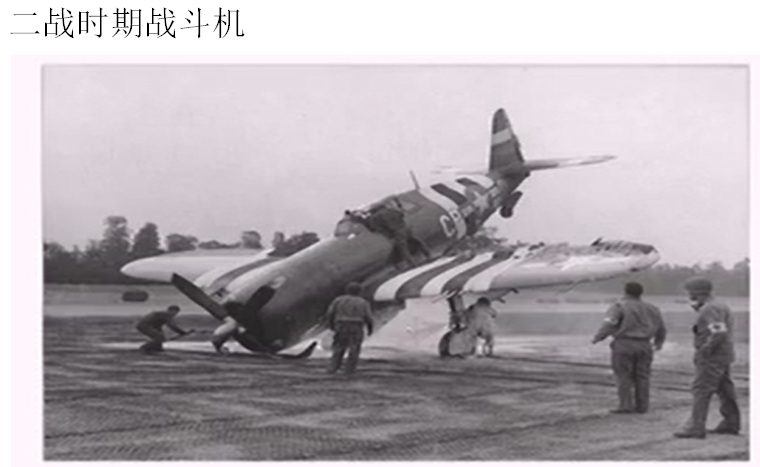
\includegraphics[width=10cm]{WW2Screenshot_2021-04-07_2220541.jpg}
\strut
\end{minipage}}

我：你看看下面例子，便会更了解随机抽样的重要性：

\framebox{%
\begin{minipage}[t]{0.97\columnwidth}\raggedright
只挑选合“味道”的来做比较 (Picking
cherries)\\
%\href{文件:儿童MA.1.jpg}{400px}}\\
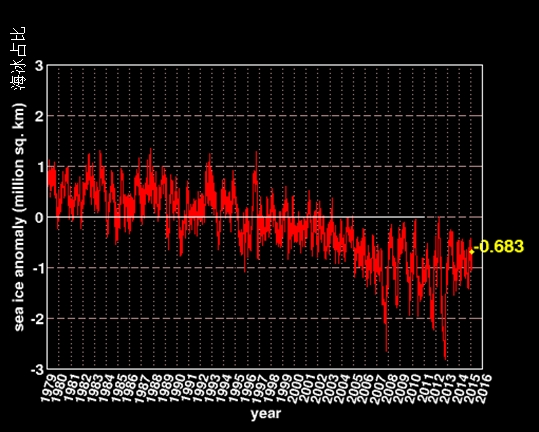
\includegraphics[width=10cm]{儿童MA1.jpg}\\
从上面80年代到现在全球海洋冰量的统计很明显看到地球在不断地暖软化。但你还可以抽两个时间，例如：2012年4月份的冰量比1988年6月份多，来说明“全球变冷”！
\strut
\end{minipage}}


孩子对统计分析好像越来越感兴趣。\\
我：现在你开始知道什么叫统计了吗？明天可以跟老师讲故事了吗？\\
孩子追着问：可不可以再给我一个练习题？我觉得这统计学也没什么困难，我还可以把你给我的那些题目拿给我同桌小李试试，看他懂不懂(男孩总是要当英雄，出风头)。\\
我：好啊。下面的身高统计数据，请你用刚才的方式来汇总一下，看看你学会没有？\\

\hypertarget{ux540dux5987ux5973ux53c2ux52a0ux67d0ux79cdux75beux75c5ux7814ux7a76ux5979ux4eecux7684ux8eabux9ad8ux4ee5ux7c73ux8ba1ux5206ux522bux4e3a}{%
\subsubsection{20名妇女参加某种疾病研究，她们的身高(以米计)分别为：}\label{ux540dux5987ux5973ux53c2ux52a0ux67d0ux79cdux75beux75c5ux7814ux7a76ux5979ux4eecux7684ux8eabux9ad8ux4ee5ux7c73ux8ba1ux5206ux522bux4e3a}}

1.52, 1.60, 1.57, 1.52, 1.60, 1.75, 1.73, 1.63, 1.55, 1.63\\
1.65, 1.55, 1.65, 1.60, 1.68, 2.50, 1.52, 1.65, 1.60, 1.65

他便拿着纸，用刚才学过的方式计算中位数、三分系数等，蛮有自信地画图、交卷。\\
我：你认识2.5米高的女性吗？\\
小孩：好像没有。\\
我：所以里面的2.50
肯定是不对。你为什么没有疑问，直接去做？统计分析必须要判断数据是否正确、是否合理。\\
如果数据本身不可靠，那么怎么分析都没用，我们称之为``垃圾进，垃圾出''（Garbage
in, Garbage out）。\\
我：有很多人利用图表误导读者，所以我们看``统计专家''的分析报告时要小心。\\

\hypertarget{ux7f8eux56fdux4e2dux897fux90e8ux623fux4ef7ux8d8bux52bfux56fe}{%
\subsubsection{美国中西部房价趋势图}\label{ux7f8eux56fdux4e2dux897fux90e8ux623fux4ef7ux8d8bux52bfux56fe}}

%\href{文件:美国中西部房价.jpg}{700px}

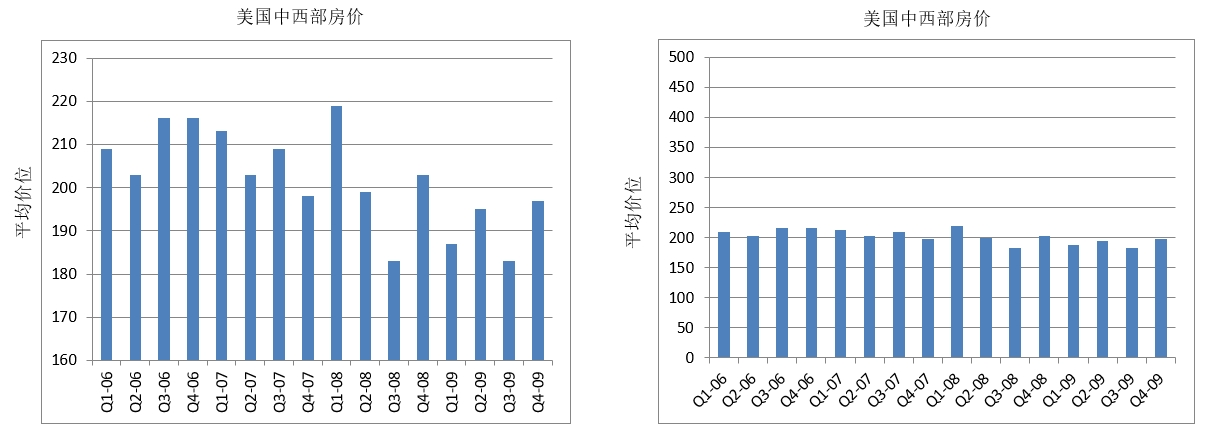
\includegraphics[width=10cm]{美国中西部房价.jpg}

上图是1906年到1909年美国中西部每个季度的房价。如果我们看右面那个柱状图，你会认为房价波动很大。但是如果同样这组数据看左面柱状图的话，你就会觉得没有太多变化。所以我们要注意看左面坐标有没有标明数字。不应该仅仅看图。\\
虽然数据都一样，但如图形不一样，传达的信息便完全不同。\\
孩子：你说的我都懂，很简单。\\
我：有很多用统计分析骗人的故事。你不是说要今年暑假找暑期工赚钱，下面是一个去工厂找工作的故事：\\
\{\textbar{} class="wikitable" \textbar{}-
\textbar{}小李刚中学毕业去工厂找工作。\\
小李问人事：工厂员工薪水是多少？\\
人事部经理面带笑容地跟他说：我们工厂员工平均月收入大概3300。\\
小李进了工厂后，才发现绝大部分的工人月薪是2000。有多年经验的工人才可以拿到2400。但有少数的管理层的平均月薪是25,000。

%\href{文件:人数薪水.jpg}{500px}

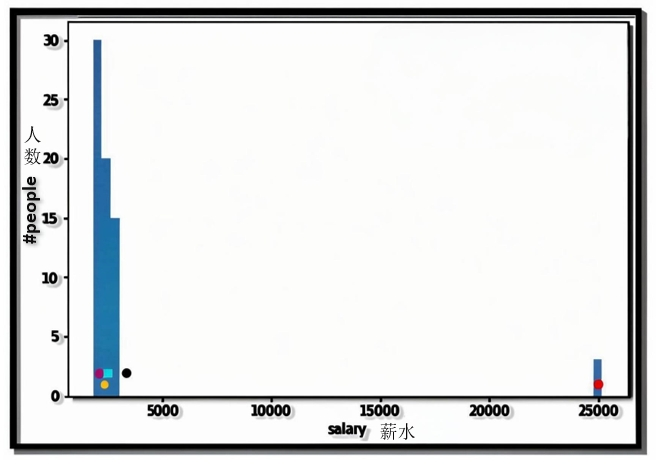
\includegraphics[width=10cm]{人数薪水.jpg}

工厂员工平均收入是每月3309，所以人事部经理没有``骗''小李。

\textbar{}\}

\hypertarget{ux5206ux6790ux4f8bux5b50ux8fdeux7eedux4e0eux5206ux7ec4ux6570ux636e}{%
\subsection{分析例子：连续与分组数据}\label{ux5206ux6790ux4f8bux5b50ux8fdeux7eedux4e0eux5206ux7ec4ux6570ux636e}}

第二天，孩子乖乖地来找我。\\
他说：爸爸，今天我跟老师说了你的工作是做统计分析，老师听到就发我一些高年级的生物实验数据，希望帮他做些分析，看两类实验有没有差异。你可以帮忙吗？\\

\hypertarget{ux8695ux8c46ux690dux7269-ux53ccux6837ux672ctux68c0ux9a8c}{%
\subsubsection{蚕豆植物
------双样本T检验}\label{ux8695ux8c46ux690dux7269-ux53ccux6837ux672ctux68c0ux9a8c}}

以下数据比较10个剪枝和10个生根样本中某化学物质的浓度：\\
剪枝:53, 58, 48, 18, 55, 42, 50, 47, 51, 45\\
生根:36, 33, 40, 43, 25, 38, 41, 46, 34, 29\\
~\\
我:你可以同样用昨天学过的方法（如柱状图）比较两组数。\\
孩子就按这个汇总了两个实验数据的分布。\\
%\url{文件:图片61-1.1.png}

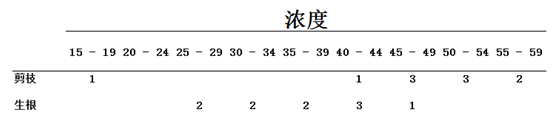
\includegraphics[width=10cm]{图片61-11.png}

我：你应该也看出剪枝样本有一个很明显的异常点------18。你应该问老师，18是否错误还是值得相信的数？如果18是不对，你就很明显看到上面剪枝的平均浓度比下面生根高。如果不能``看''出来就可以用``双样本T''检验比较两组数据是否有显著差异。但是如果有刚刚那种异常点，如直接用双样本T分析，因为第一组数据被那个18拉低了，得出结果是两组没有显著差异。所以还是直接看数据的分布更实在。\\
我：我们在统计学可以使用假设检验（注），其中包括双样本T检验比较、方差分析(ANOVA)等，就是针对这类统计数据分析。但是在你这个实验数据，从画图一眼都能看出有显著区分，就不需要再采用假设检验，因采用那些方法不会得出额外的信息。\\
我接着跟他说:有些时候统计数据不是连续数据，像学生成绩、浓度、高度等，而是分组数据。例如下面这些国外人种眼睛颜色与头发颜色的数据，这种数据我们就需要用列联表
(Contingency Table) 来识别这两个变量之间有没有关系。\\

\hypertarget{ux5934ux53d1ux548cux773cux775bux989cux8272ux7684ux4e0dux540cux7ec4ux5408}{%
\subsubsection{头发和眼睛颜色的不同组合}\label{ux5934ux53d1ux548cux773cux775bux989cux8272ux7684ux4e0dux540cux7ec4ux5408}}

592人的头发和眼睛颜色的不同组合：

\resizebox{\linewidth}{!}{

\renewcommand{\arraystretch}{1.5}

\begin{tabular}{|c|c|c|c|c|}
\hline
表1&\multicolumn{4}{|c|}{头发颜色 }\\
\hline
眼睛颜色&黑&深褐&红&金\\
\hline
棕&68&119&26&7\\
\hline
蓝&20&84&17&94\\
\hline
淡绿褐&15&54&14&10\\
\hline
绿&5&29&14&16\\
\hline
\end{tabular}
}


如果我们利用表1的数，把它那些每一行、每一列进行求和，我们可以看见每列或者每行的分析结果。例如棕色眼睛的占大多数，但金发例外，金发的大部分是蓝眼睛。其实也看到金头发的那列跟其他的一些分布很不一样。比如我们看每行的话，也可以看到棕色眼睛跟蓝眼睛的数量差不多。但在金头发和黑头发的列分布就不一样了。统计分析的卡方检验也可以帮我们分析分组数据间有没有相关。但刚才这类简单4×4数据表，计算出表3列联表便足够，卡方检验没有带来更多有用信息。\\
\textbf{实际(Obs.) 数量表}:

\resizebox{\linewidth}{!}{

\renewcommand{\arraystretch}{1.5}

\begin{tabular}{|c|c|c|c|c|c|}
\hline
表2&\multicolumn{5}{|c|}{头发颜色 }\\
\hline
眼睛颜色&黑&深褐&红&金&总计\\
\hline
棕&68&119&26&7&220\\
\hline
蓝&20&84&17&94&215\\
\hline
淡绿褐&15&54&14&10&93\\
\hline
绿&5&29&14&16&64\\
\hline
总计&108&286&71&127&592\\
\hline
\end{tabular}

}


\textbf{实际(Obs.) vs 预计(Exp.)数量表 Contingency Table}:

\resizebox{\linewidth}{!}{

\renewcommand{\arraystretch}{1.5}

\begin{tabular}{|c|c|c|c|c|c|c|c|c|c|}
\hline
表3&\multicolumn{8}{|c|}{头发颜色 }&\:\\
\hline
\:&\multicolumn{2}{|c|}{黑}&\multicolumn{2}{|c|}{深褐}&\multicolumn{2}{|c|}{红}&\multicolumn{2}{|c|}{金}&\:\\
\hline
眼睛颜色&Obs.&Exp.&Obs.&Exp.&Obs.&Exp.&Obs.&Exp.&Total\\
\hline
棕&68&40&119&106&26&26&7&47&220\\
\hline
蓝&20&39&84&104&17&26&94&46&215\\
\hline
淡绿褐&15&17&54&45&14&11&10&20&93\\
\hline
绿&5&12&29&31&14&8&16&14&64\\
\hline
总计&\multicolumn{2}{|c|}{108}&\multicolumn{2}{|c|}{286}&\multicolumn{2}{|c|}{71}&\multicolumn{2}{|c|}{127}&592\\
\hline
\end{tabular}

}

注：双样本T检验、方差分析(ANOVA)、卡方检验等都属于假设检验(Hypothesis
Testing)，附件里用某卡方检验为例，说明如何利用计算出的p值做判断。

\hypertarget{ux603bux7ed3}{%
\subsection{总结}\label{ux603bux7ed3}}

分析数据前应先用图或数量描述数据分布，包括：

\begin{itemize}
\tightlist
\item
  平均值、中位数、四分位数(Q1、Q2、Q3)、众数
\item
  柱状图、箱线图、茎叶图等
\end{itemize}

下表总结本章对应描述性统计的注意项：

\resizebox{\linewidth}{!}{

\renewcommand{\arraystretch}{1.5}


\begin{tabular}{|c|c|}
\hline
步骤&上面实例 \\
\hline
\:&这些数字代表什么?什么单位（角度、还是距离）？ \\
\hline
策划收集数据&怎样取样？避免取样偏差 \\
\hline
确保数据质量&2.5米高女性？异常数据？ \\
\hline
初步数据分析（描述性)&平均值、四分位数(Q1、Q2、Q3)、柱状图、箱线图 \\
\hline
数据分析&如果能简单看出来有显著差异，便不需要用假设检验，或其他统计分析方法\\
\hline
解读、沟通结果&当我们读统计分析报告要小心，注意是否被骗 \\
\hline
\end{tabular}

}

了解每个变量的分布后，便可按数据，分析变量间的关系：


\resizebox{\linewidth}{!}{

\renewcommand{\arraystretch}{1.5}


\begin{tabular}{|c|c|}
\hline
注意项 & 例子 \\
\hline
分析两组数据间有没有显著差异。如果能简单看出分布的差异，比只用假设检验更有洞察& 双样本T检验 \\
\hline
头发眼睛颜色 列联表 & \:\\
\hline
确保数据质量&2.5米高女性？异常数据？ \\
\hline
\end{tabular}

}



从以上例子看到要有效分析，应按数据本质挑选合适的方法，而不是墨守成规，像机器人一样按规定分析。

\hypertarget{ux9644ux4ef6}{%
\section{附件}\label{ux9644ux4ef6}}

\hypertarget{ux5982ux4f55ux753bux830eux53f6ux56festem-and-leaf-plot}{%
\subsection{如何画茎叶图(Stem and Leaf
Plot)}\label{ux5982ux4f55ux753bux830eux53f6ux56festem-and-leaf-plot}}

以文中20名学生在数学考试分数为例：

\begin{enumerate}
\tightlist
\item
  把分数从小到大排序
\item
  从上而下画一直线
\item
  第一个数30，左边写3，右面写0（叶）
\item
  排第二是35，因5大于0-4，新一行，左边写3，右面写5（叶）
\item
  37，因7属于5\textasciitilde{}9，所以同一行，在5右面写7（叶）
\item
  最终便可以简单利用数目字形成一个横放的直方图
\end{enumerate}

\hypertarget{ux7bb1ux7ebfux56fe-box-and-whisker-plot}{%
\subsection{箱线图 (Box and Whisker
Plot)}\label{ux7bb1ux7ebfux56fe-box-and-whisker-plot}}

\href{文件:BoxWhiskerScreenshot_2021-08-02_214603.1.jpg}{500px}

箱线图包括5个数：

\begin{itemize}
\tightlist
\item
  Minimum 最少 (Q0 )
\item
  1st Quartile (Q1 , 25 percentile) 箱子的左面边线
\item
  Medium 中位数 (Q2 , 50 percentile) 箱子中间的线
\item
  3rd Quartile (Q3 , 75 percentile) 箱子的右面边线
\item
  Maximum 最大 (Q4 , 100 percentile)
\end{itemize}

有些箱线图直接把两头指到最大与最少，不展示离散点 (Outliers)。

Interquartile range (IQR) = Q3 - Q1

\hypertarget{ux5361ux65b9ux68c0ux9a8cchi-square-test}{%
\subsection{卡方检验(Chi Square
test)}\label{ux5361ux65b9ux68c0ux9a8cchi-square-test}}

研究三家医院(A、B、C)在3类最终导致患者死亡感染的主因（外科手术Surgical
Site、肺炎Pneumonia、血液Bloodstream），分布是否有显著差异？

%\href{文件:4chiSquareDataScreenshot_2022-07-24_110053.jpg}{文件:4chiSquareDataScreenshot
%2022-07-24 110053.jpg}\\

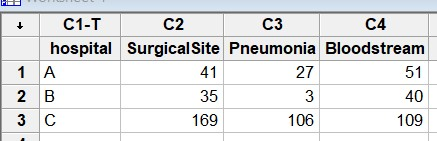
\includegraphics[width=10cm]{4chiSquareDataScreenshot_2022-07-24_110053.jpg}

\{\textbar{} class="wikitable" \textbar{}-
\textbar{}\textbf{假设检验的步骤}

零假设: A哪家医院与死亡主因没有显著关系\\
挑选对应的检验方法后，可以利用工具计算出的P值来判断。\\
::如果P值大于0.05，就不能拒绝零假设。\\
\href{文件:6chiSquareTstResultScreenshot_2022-07-24_103606-1.jpg}{500px}\\
卡方检验得出P值等于零，所以可以拒绝零假设，医院与感染主因有关系。
\textbar{}\}

\begin{itemize}
\tightlist
\item
  如不用工具，也可以手工计算卡方值(Chi-square)，首先使用以下公式计算每个列联表的预计值E(Expected
  Value)，
\end{itemize}

\(E = \frac{(row \ sum) * (column \ sum)} {grand \ total}\)

再用下面公式从预计值与实际值O(Observed value),计算卡方值 ：

\(\chi ^2 = \sum \frac{(O - E)^2} {E}\)

\begin{itemize}
\tightlist
\item
  计算得出卡方值 = 30.696（注），比关键值9.5高
\end{itemize}

\begin{description}
\item[]
(对应 DF=4 (=(3-1)*(3-1))
，\(\alpha = 0.05\)，从\(\chi ^2\)统计表得出9.5)，\\
\end{description}

所以拒绝零假设，医院(Hospitals) 与感染种类(Infections)之间相关。\\
:注：接近工具自动算出的30.755。

\hypertarget{ux53c2ux8003-references}{%
\section{参考 References}\label{ux53c2ux8003-references}}

\begin{enumerate}
\tightlist
\item
  Guttag, John V. \emph{Introduction to computation and programming
  using Python.} (MIT Press , 2021)\\
\item
  Chatfield, Chris. \emph{Problem Solving: a statistician's guide.} 2/e
  (Chapman \& Hall, 1995)\\
\item
  Bluman, Allan. \emph{Elementary Statistics.} 10/e (McGraw - Hill ,
  2018)\\
\end{enumerate}

